\documentclass[margin=1mm]{standalone}
\usepackage[utf8]{inputenc}
\usepackage{amsmath}
\usepackage{amsfonts}
\usepackage{amssymb, bm}
\usepackage{tikz}
\usetikzlibrary{calc,arrows,positioning,shapes,shapes.gates.logic.US,trees, backgrounds}
\usetikzlibrary{fit, positioning}

\begin{document}
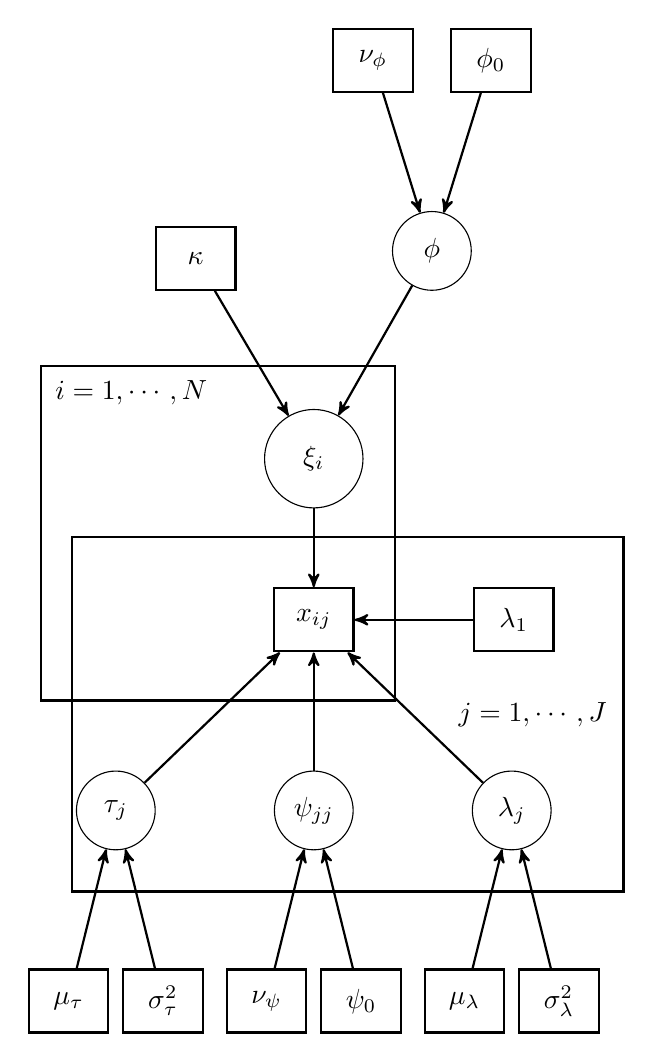
\begin{tikzpicture}[auto,scale=3,
	latent/.style={circle,draw,text badly centered, inner sep=2pt,minimum size=12.5mm},
	error/.style={circle,draw,text badly centered, inner sep=2pt,minimum size=10mm},
	manifest/.style={text centered, rectangle,draw,thick,inner sep=3pt,minimum height=8mm, minimum width=8mm, text width= 8 mm},
	  plate/.style={draw, shape=rectangle,thick, minimum height=4.25cm, minimum width=4.5cm, text width=1cm, align=right, inner sep=10pt, inner ysep=10pt, append after command={node[below right= 3pt of \tikzlastnode.north west] {#1}}},
	  plate2/.style={draw, shape=rectangle,thick, minimum height=4.5cm, minimum width=7cm, text width=1cm, align=right, inner sep=5pt, inner ysep=8pt, append after command={node[left= 3pt of \tikzlastnode.east] {#1}}},
	manifestRot/.style={text centered, rectangle, draw, thick,inner sep=3pt, minimum width=7mm, text width= 7mm, minimum height=15},
	manifestfront/.style={rectangle,draw,thick,inner sep=0pt,minimum size=12mm, fill=white},
	ghost/.style={rectangle, inner sep=0pt,text centered,    minimum height=0mm, minimum width=5mm, text width= 5 mm},
	lcorr/.style={<->,>=stealth', bend right=40},
	rcorr/.style={<->,>=stealth', bend left=40},
	fcorr/.style={<->,>=stealth', bend left=40},
	ofcorr/.style={<->,>=stealth', bend right=60},
	ofcorr2/.style={<->,>=stealth', bend left=60},
	intercept/.style={regular polygon,
        regular polygon sides=3,draw,thick,inner sep=0pt,minimum size=10mm},
	mean/.style={regular polygon,regular polygon sides=3,draw,thick,inner sep=0pt,minimum size=10mm},
	paths/.style={->, thick, >=stealth'},
	variance/.style={<->, thick, >=stealth', bend left=270, looseness=2},
	varianceTop/.style={<->, thick, >=stealth', bend right=270, looseness=2},
	unique/.style={<->, thick, >=stealth', loop below=270, looseness=8},
	factvar/.style={<->, thick, >=stealth', loop right=270, looseness=8}
	] % End Creating Path Model Pieces
\tikzset{mystyle/.style={->,double=black}}


% person model
\node [manifest] at (0,0) (x) {$x_{ij}$};
\node [latent]     [above = 1cm of x] (t) {$\xi_i$};
\node [manifest]   [above = 1.5cm of t,  xshift=-1.5cm] (k)   {$\kappa$};
\node [error]      [above = 1.5cm of t,  xshift= 1.5cm] (phi)   {$\phi$};
  \node [manifest] [above = 1.5cm of phi, xshift=-.75cm] (phi1) {$\nu_{\phi}$};
  \node [manifest] [above = 1.5cm of phi, xshift= .75cm] (phi2) {$\phi_0$};
\node [manifest]   [right = 1.5cm of x] (l1) {$\lambda_1$};
\node [error]      [below = 1.5cm of x] (ej) {$\psi_{jj}$};
  \node [manifest] [below = 1.5cm of ej, xshift=-.6cm] (ej0) {$\nu_{\psi}$};
  \node [manifest] [below = 1.5cm of ej, xshift= .6cm] (ej1) {$\psi_0$};
\node [error]      [right = 1.5cm of ej] (l2) {$\lambda_j$};
  \node [manifest] [below = 1.5cm of l2, xshift=-.6cm] (l20) {$\mu_\lambda$};
  \node [manifest] [below = 1.5cm of l2, xshift= .6cm] (l21) {$\sigma^2_{\lambda}$};
\node [error]      [left = 1.5cm of ej] (t0) {$\tau_{j}$};
  \node [manifest] [below = 1.5cm of t0, xshift=-.6cm] (t00) {$\mu_{\tau}$};
  \node [manifest] [below = 1.5cm of t0, xshift= .6cm] (t01) {$\sigma^2_{\tau}$};  

\node [plate={$i=1, \cdots, N$}] [right= -4cm of x, yshift=1.1cm] (p) {};
\node [plate2={$j=1, \cdots, J$}] [right= -3.6cm of x, yshift=-1.2cm] (p2) {};


% paths
\draw[paths] (t)  -- (x);
\draw[paths] (k) -- (t);
\draw[paths] (phi) -- (t);
\draw[paths] (l1) -- (x);
\draw[paths] (l2) -- (x);
\draw[paths] (ej) -- (x);
\draw[paths] (t0) -- (x);
\draw[paths] (phi1) -- (phi);
\draw[paths] (phi2) -- (phi);
\draw[paths] (t00) -- (t0);
\draw[paths] (t01) -- (t0);
\draw[paths] (l20) -- (l2);
\draw[paths] (l21) -- (l2);
\draw[paths] (ej0) -- (ej);
\draw[paths] (ej1) -- (ej);
\end{tikzpicture}
\end{document}